\documentclass[12pt,a4paper,oneside]{article}
\usepackage[utf8]{vietnam}
\usepackage{amsmath}
\usepackage{amsfonts}
\usepackage{amssymb}
\usepackage{graphicx}
\usepackage[left=2cm,right=2cm,top=2cm,bottom=2cm]{geometry}
\usepackage{array}
\usepackage{fancyhdr}
\pagestyle{fancy}
\renewcommand\thesection{\Roman{section}.}
\renewcommand\thesubsection{\arabic{subsection}.}
\fancyhf{}
\rhead{{\large \textbf{Laboratory Exercise 10}}}
\lhead{Hoàng Quốc Bảo - 20194484}
\rfoot{Trang \thepage}

\usepackage{listings}
\usepackage{tcolorbox}
\usepackage{color} % tô màu cho code
\definecolor{dkgreen}{rgb}{0,0.6,0}
\definecolor{gray}{rgb}{0.5,0.5,0.5}
\definecolor{code}{rgb}{0.8,0.8,0.8}
\definecolor{mauve}{rgb}{0.58,0,0.82}
\lstset{frame=tb,
  language=[x86masm]Assembler,
  aboveskip=3mm,
  belowskip=3mm,
  showstringspaces=false,
  columns=flexible,
  basicstyle={\small\ttfamily},
  backgroundcolor=\color{gray!20!white},
  numbers=none,
  breaklines=true,
  breakatwhitespace=true,
  tabsize=3
}

\begin{document}
\section*{Assignment 3: MARSBOT RIDER}
\textbf{Mã nguồn:}
\begin{lstlisting}
.eqv HEADING 0xffff8010 # Integer: An angle between 0 and 359
 # 0 : North (up)
# 90: East (right)
 # 180: South (down)
 # 270: West (left)
.eqv MOVING 0xffff8050 # Boolean: whether or not to move
.eqv LEAVETRACK 0xffff8020 # Boolean (0 or non-0):
 # whether or not to leave a track
.eqv WHEREX 0xffff8030 # Integer: Current x-location of MarsBot
.eqv WHEREY 0xffff8040 # Integer: Current y-location of MarsBot

.text 
main: jal UNTRACK # Move to draw place
 nop
 addi $a0, $zero, 180 # Marsbot rotates 90* and start running
 jal ROTATE
 nop
 jal GO
 nop
 sleep1: addi $v0,$zero,32 # Keep running by sleeping in 3000 ms
 li $a0,3000 
 syscall
 
 addi $a0, $zero, 90 
 jal ROTATE
 nop
 jal GO
 nop
 sleep2: addi $v0,$zero,32 # Keep running by sleeping in 3000 ms
 li $a0,3000 
 syscall
 
 startdraw:  
 b1: jal TRACK
 nop
 addi $a0, $zero, 180
 jal ROTATE
 nop
 jal GO
 nop
 sleep3: addi $v0,$zero,32 # Keep running by sleeping in 6000 ms
 li $a0,7000 
 syscall
 jal UNTRACK # keep old track
 nop
 jal TRACK # and draw new track line
 nop
 
b2: addi $a0, $zero, 90
 jal ROTATE
 nop
 jal GO
 nop
 sleep4: addi $v0,$zero,32 # Keep running by sleeping in 3000 ms
 li $a0,3000 
 syscall
 jal UNTRACK # keep old track
 nop
 jal TRACK # and draw new track line
 nop
 
 b3: addi $a0, $zero, 0
 jal ROTATE
 nop
 jal GO
 nop
 sleep5: addi $v0,$zero,32 # Keep running by sleeping in 3000 ms
 li $a0,3000 
 syscall
 jal UNTRACK # keep old track
 nop
 jal TRACK # and draw new track line
 nop
 
 b4: addi $a0, $zero, 270
 jal ROTATE
 nop
 jal GO
 nop
 sleep6: addi $v0,$zero,32 # Keep running by sleeping in 3000 ms
 li $a0,3000 
 syscall
 jal UNTRACK # keep old track
 nop
 jal TRACK # and draw new track line
 nop
 
 b5: addi $a0, $zero, 0
 jal ROTATE
 nop
 jal GO
 nop
 sleep7: addi $v0,$zero,32 # Keep running by sleeping in 3000 ms
 li $a0,1000 
 syscall
 jal UNTRACK # keep old track
 nop
 jal TRACK # and draw new track line
 nop
 
##########
b6: addi $a0, $zero, 90
 jal ROTATE
 nop
 jal GO
 nop
 sleep8: addi $v0,$zero,32 # Keep running by sleeping in 3000 ms
 li $a0,3000 
 syscall
 jal UNTRACK # keep old track
 nop
 jal TRACK # and draw new track line
 nop
 
 b7: addi $a0, $zero, 0
 jal ROTATE
 nop
 jal GO
 nop
 sleep9: addi $v0,$zero,32 # Keep running by sleeping in 3000 ms
 li $a0,3000 
 syscall
 jal UNTRACK # keep old track
 nop
 jal TRACK # and draw new track line
 nop
 
 b8: addi $a0, $zero, 270
 jal ROTATE
 nop
 jal GO
 nop
 sleep10: addi $v0,$zero,32 # Keep running by sleeping in 3000 ms
 li $a0,3000 
 syscall
 jal UNTRACK # keep old track
 nop
end_main:
 
#-----------------------------------------------------------
# GO procedure, to start running
# param[in] none
#-----------------------------------------------------------
GO: li $at, MOVING # change MOVING port
 addi $k0, $zero,1 # to logic 1,
 sb $k0, 0($at) # to start running
 nop 
 jr $ra
 nop
#-----------------------------------------------------------
# STOP procedure, to stop running
# param[in] none
STOP: li $at, MOVING # change MOVING port to 0
 sb $zero, 0($at) # to stop
 nop
 jr $ra
 nop
#-----------------------------------------------------------
# TRACK procedure, to start drawing line 
# param[in] none
#----------------------------------------------------------- 
TRACK: li $at, LEAVETRACK # change LEAVETRACK port
 addi $k0, $zero,1 # to logic 1,
 sb $k0, 0($at) # to start tracking
 nop
 jr $ra
 nop 
#-----------------------------------------------------------
# UNTRACK procedure, to stop drawing line
# param[in] none
#----------------------------------------------------------- 
UNTRACK:li $at, LEAVETRACK # change LEAVETRACK port to 0
 sb $zero, 0($at) # to stop drawing tail
 nop
 jr $ra
 nop
#-----------------------------------------------------------
# ROTATE procedure, to rotate the robot
# param[in] $a0, An angle between 0 and 359
# 0 : North (up)
# 90: East (right)
# 180: South (down)
# 270: West (left)
#-----------------------------------------------------------
ROTATE: li $at, HEADING # change HEADING port
 sw $a0, 0($at) # to rotate robot
 nop
 jr $ra
 nop
\end{lstlisting}
\pagebreak
\textbf{Giải thích:\\\\}
\textbf{Mục tiêu:} Ta cần vẽ chữ B.
\begin{itemize}
\item Đầu tiên, chúng ta dùng các lệnh sau để di chuyển Marsbot về địa điểm cần vẽ.
\begin{center}
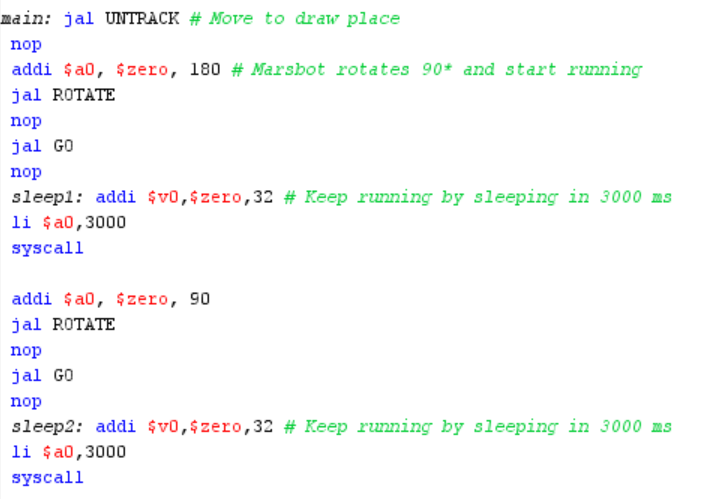
\includegraphics[scale=1]{1}
\end{center}
\textbf{Kết quả thực hiện:}
\begin{center}
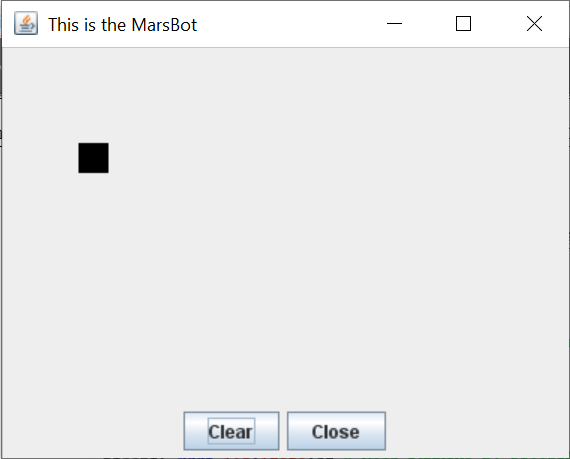
\includegraphics[scale=1]{2}
\end{center}
\pagebreak
\item Tiếp theo, ta dùng các lệnh sau để vẽ nét đầu tiên của chữ B.
\begin{center}
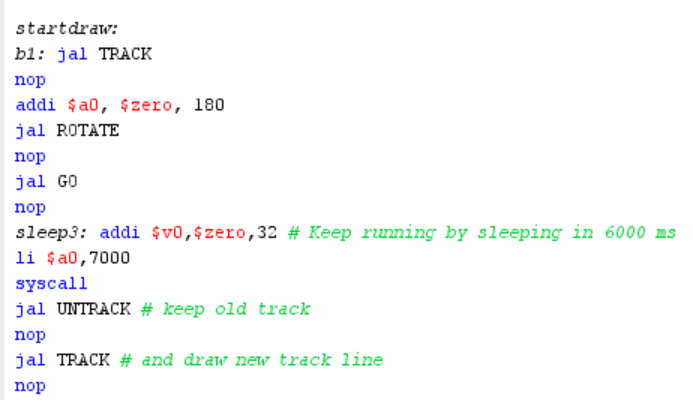
\includegraphics[scale=1]{3}
\end{center}
\textbf{Kết quả thực hiện:}
\begin{center}
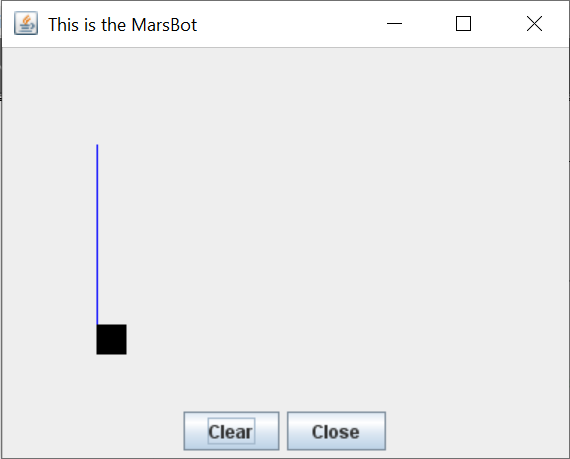
\includegraphics[scale=1]{4}
\end{center}
\pagebreak
\item Tương tự cho các nét sau
\begin{center}
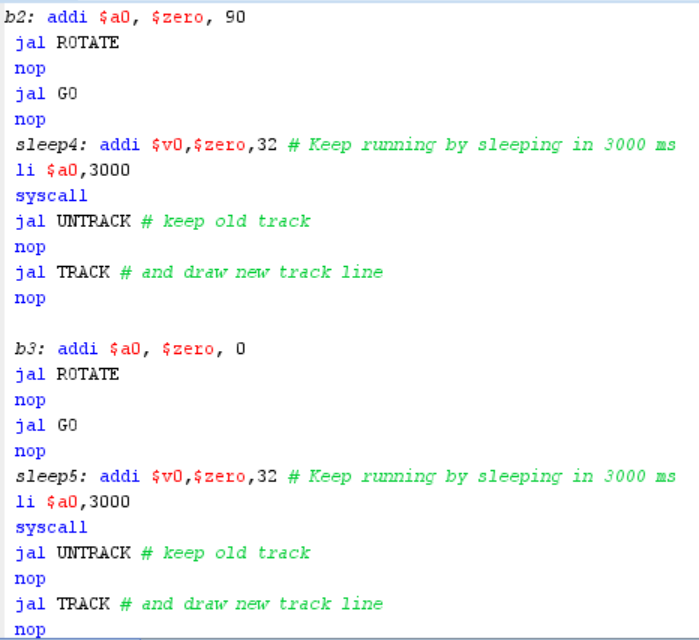
\includegraphics[scale=1]{5}
\end{center}
\textbf{Kết quả thực hiện:}
\begin{center}
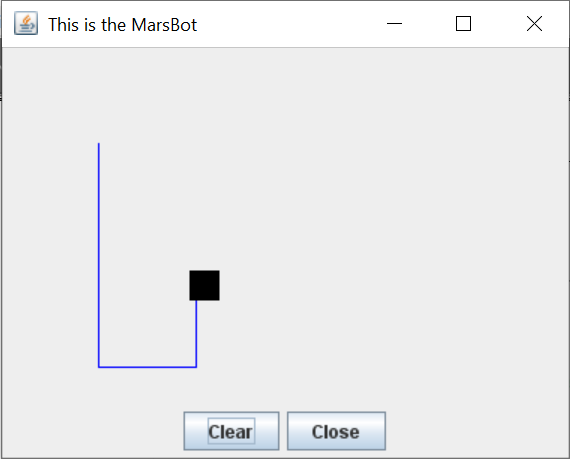
\includegraphics[scale=1]{6}
\end{center}
\pagebreak
\item Các bước sau tương tự.\\\\
\textbf{Kết quả thực hiện:}
\begin{center}
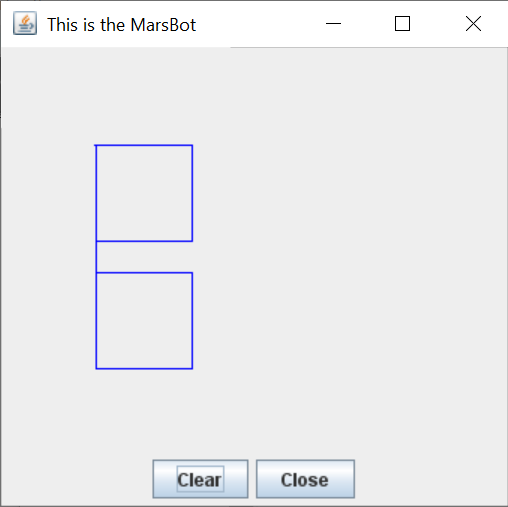
\includegraphics[scale=1]{7}
\end{center}
\end{itemize}
\pagebreak
\section*{Assignment 4: KEYBOARD and DISPLAY MMIO}
\textbf{Mã nguồn:}
\begin{lstlisting}
.eqv KEY_CODE 0xFFFF0004 # ASCII code from keyboard, 1 byte
.eqv KEY_READY 0xFFFF0000 # =1 if has a new keycode ?
 # Auto clear after lw

.eqv DISPLAY_CODE 0xFFFF000C # ASCII code to show, 1 byte
.eqv DISPLAY_READY 0xFFFF0008 # =1 if the display has already to do
 # Auto clear after sw

.text
 li $k0, KEY_CODE
 li $k1, KEY_READY
 
 li $s0, DISPLAY_CODE
 li $s1, DISPLAY_READY

loop: nop
 
WaitForKey: lw $t1, 0($k1) # $t1 = [$k1] = KEY_READY
 nop
 beq $t1, $zero, WaitForKey # if $t1 == 0 then Polling
 nop
 #-----------------------------------------------------
ReadKey: lw $t0, 0($k0) # $t0 = [$k0] = KEY_CODE
 nop
QuitKey:
 beq $t0, 'b', quit
 nop
 #-----------------------------------------------------
WaitForDis: lw $t2, 0($s1) # $t2 = [$s1] = DISPLAY_READY
 nop
 beq $t2, $zero, WaitForDis # if $t2 == 0 then Polling 
 nop 
 #-----------------------------------------------------
Encrypt: addi $t0, $t0, 4 # change input key
 #-----------------------------------------------------
ShowKey: sw $t0, 0($s0) # show key
 nop 
 #----------------------------------------------------- 
 j loop
 nop
 quit:
\end{lstlisting}
\pagebreak
\textbf{Giải thích:}\\
- So với mã nguồn gốc, ta cần thay đổi giá trị mã hoá từ 1 sang chữ số cuối MSSV \textit{(4)}.
\begin{center}
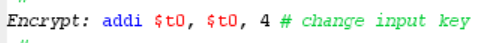
\includegraphics[scale=1]{8}
\end{center}
- Và bổ sung thêm đoạn mã dừng chương trình khi gặp kí tự đầu tiên trong tên \textit{(b)}.
\begin{center}
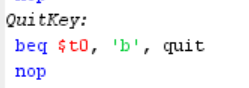
\includegraphics[scale=1]{10}
\end{center}
\textbf{Kết quả thực hiện:}
\begin{center}
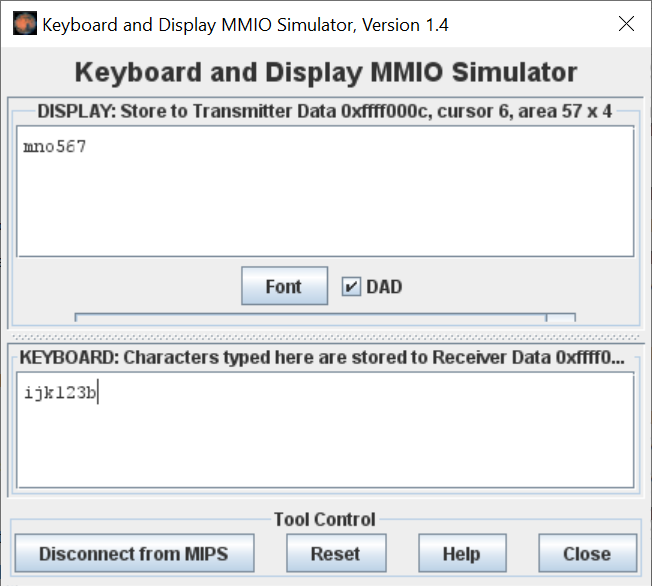
\includegraphics[scale=1]{9}
\end{center}
\end{document}